%%%%%%%%%%%%%%%%%%%%%
%								%
%	ESTADO DEL ARTE				%
%								%
%%%%%%%%%%%%%%%%%%%%%
\chapter{Estado del Arte}\label{cap:estadoArte}



%Por definición \textit{e-Commerce}: Transacción comercial electrónica, así como sobre Internet.
%
%Vender y realizar transacciones como estas se pueden hacer gracias a \textit{World Wide Web}, el cual es una convinación global de \textit{links}, información, paginas \textit{web} y \textit{e-Commerce websites}.
%
%Con el fin de considerar 

\section{Categorías de \ecommerce}

Tecnología digital avanzada, combinada con las empresas y los clientes de estas tecnologías, impulsan \ecommerce. De igual forma que las tecnologías digitales, \ecommerce no pudo alcanzar su meta en un movimiento. En cuanto a las empresas y clientes, \ecommerce de diferentes tipos y niveles implica diferentes oportunidades \cite{zheng2009fundamentals}.

En relación a categorías de transacciones, \ecommerce se divide en 5 tipos:
\begin{figure}[h!]
	\centering
	\includegraphics[width=0.5\textwidth]{figuras/ecommerce_types.png}
	\caption{Categorias de \ecommerce.}
\end{figure}

\begin{itemize}
	\item \textbf{\btob}. Es simplemente definido como \ecommerce entre compañías. Este es el tipo de \ecommerce que tiene que ver con las relaciones entre y dentro de los negocios. Cerca del 80\% de \ecommerce que existe, corresponde a esta categoría, y cada vez son mas los expertos que predicen que \btob \ecommerce continuara su crecimiento a una velocidad mayor que el segmento \btoc.

%B2B e-commerce is simply defined as e-commerce between companies. This is the type of e-commerce that deals with relationships between and among businesses. About 80\% of e-commerce is of this type, and most experts predict that B2B ecommerce will continue to grow faster than the B2C segment.

	\item \textbf{\btoc}. En este caso, \internet utilizado por negocios y empresas para proveer bienes y servicios por sities \web a los clientes. Actualmente varios tipos de sitios \web \btoc estan repartidos por \internet para suministrar a los clientes una variedad de bienes y servicios que van desde flores y libros, hasta los ordenadores y autos, etc.

	\item \textbf{\btog}.El gobierno, como administrador nacional, desempeña un papel importante en la orientación, administración y ajuste de la economía. El advenimiento de la era de \ecommerce planteó fundamentos \ecommerce las nuevas solicitudes de las funciones originales de los gobiernos. Por un lado, el gobierno debería  administrar \emarket efectivamente y prestar un mejor servicio a las empresas y al público a través de \egoverment. Por otra parte, los gobiernos, como los "grandes clientes" en economía deberían tomar iniciativa para adoptar \ecommerce y ofrecer maneras eficientes a través de invitación de licitación electrónica para las contrataciones públicas.

%Governments, as national administrators, play a significant role in guiding, administrating and adjusting economy. The advent of e-commerce age put forward Fundamentals of E-commerce the new request to the original functions of governments. Governments should administrate e-market effectively and render better service to enterprises and the public by e-government on the one hand. Governments, as the “big clients” in economy should take the lead to adopt e-commerce and offer efficient path through electronic tender invitation for government procurement on the other hand.

	\item \textbf{\gtog}.

	\item \textbf{\ctoc}. Es un comercio simple entre individuos privados o consumidores. Este tipo de \ecommerce es caracterizado por el crecimiento de mercados electrónicos y las subastas \online, particularmente en industrias verticales donde empresas/negocios pueden pujar por lo que quieren de entre varios proveedores.
%Consumer-to-consumer e-commerce or C2C is simply commerce between private individuals or consumers. This type of e-commerce is characterized by the growth of electronic marketplaces and online auctions, particularly in vertical industries where firms/businesses can bid for what they want from among multiple suppliers.

	\item \textbf{\mcommerce}.
	
\end{itemize}

\section{\keyelements de un sitio \ecommerce \cite{inbook_ecommerce_keyelements}}

\subsection{Domain y Hosting}
\subsection{Diseño}
El diseño del sitio es el principal elemento en determinar si el visitante se queda o se va.

\subsection{\usability}
\subsection{conversion}
\subsection{\checkout}
\subsection{Taking Payments}
\subsection{Product Pages}
\subsection{On-Site SEO (Search Engine Optimization)}
\subsection{Content Management System \% Automation}
\subsection{Key \ecommerce Features}
\subsection{Operation \% Order Management}
\subsection{Information Pages}
\subsection{\security, \trust \& Testimonials}

\trust y \familiarity influencian \ecommerce, como insinúa \luhmanntheory. Especialmente los datos muestran que tanto \trust en un vendedor \internet y \familiarity con el vendedor y sus procedimientos influencian dos aspectos distintos de \ecommerce en sitios de venta de libros: \inquiry y \purchase. La influencia de la  \familiarity y \trust son especialmente fuertes en intenciones  de las personas para \purchase. Segundo, los datos muestran que \trust y \familiarity son claramente diferentes construcciones, y la \trust es significativamente afectada por \familiarity, y no solo por la social disposición de la gente para \trust. El modelo de investigación muestra que  \ecommerce puede ser evaluado en el contexto de un ambiente social complejo basado en \luhmanntheory. Bajo tales circunstancias , tanto \trust como \familiarity influencian intenciones de comportamiento\cite{gefen2000commerce}.

\security influencia \trust. Por ejemplo, en el caso de \amazon, una persona \familiarity con el concepto de \secureintcom podría permitir que se entreguen creencias específicas relativas a la medida de seguridad que ellos esperan del vendedor (\trust)\cite{gefen2000commerce}.

\ebay realizo un estudio en donde demostró que la reputación \ecommerce de un vendedor es un determinante, aunque no un determinante principal, del precio que los vendedores recibían en sus subastas. En ausencia de otros, recursos mas directos de información del producto, un comprador en \internet debe confiar en la precisión de la descripción del producto del vendedor y la confiabilidad de la entrega del producto del vendedor para decidir si, y cuanto esta dispuesto a ofertar por el bien. Dicho de otra manera, la reputación del vendedor se convierte en una consideración en la voluntad del comprador para hacer una oferta en el articulo de la subasta. El resultado empírico muestra que un \seller con una mejor reputación puede esperar recibir ofertas superiores para sus \itemscommerce subastados. Sin embargo, aunque la reputación es una determinante estadisticamente significativa, su impacto tiende a ser pequeño\cite{melnik2002does}.

En este sentido, los nuevos \seller de subasta en el \websites pueden considerar difícil competir con los \sellers existentes quienes tienen establecida una reputación positiva. Ademas, en la ausencia de un mecanismo que permitan que los \ratings sean transferidos entre sitios, un \seller quien ya tiene un alto \rating en un \website de subastas \online puede enfrentar un costo en cambiar a otro \website de subastas \online. \textit{Reputación} obviamente provee algunos beneficios para los \consumers buscando  la \internet por \itemscommerce para los cuales realizar una oferta. Sin embargo, tal \textit{reputación} puede también implicar algunos costos a los \consumers, si el desarrollo de reputación para subastas \online actúa como barrera de entrada para nuevos \websites de  subastas \online  y da poder de monopolio a los \websites de subastas \online ya establecidos\cite{melnik2002does}.

\subsection{Marketing Elements}
\subsection{Analytics/reports}





Aunque no es relevante para el \framework, es importante destacar la importancia que tiene este tópico en el éxito que pueda tener una solución \ecommerce. 

%TODO


\opensource \ecommerce \shoppingcarts ofrecen muchas ventajas para \textit{small businesses}. Soluciones \opensource pueden ser desarrolladas para ajustarse a las necesidades del negociante. Ellos contienen una gran combinación de características a un mínimo costo. Y, aunque las opciones de soporte pueden ser mas limitadas que las propietarias o \textit{hosted platforms}, soluciones independientes \opensource generalmente tienen grandes comunidades de desarrolladores y socios para ayudar a los nuevos comerciantes.

\section{Ejemplos de \frameworks existentes}

Aquí hay una lista de 11 soluciones \ecommerce \opensource. El \core de todas las aplicaciones es \free. Cada aplicación tiene extensiones \free y \premium y opciones de soporte para mejorar el desarrollo de la \store.

\begin{itemize}
	\item \textbf{\nameOpenCart}. Es una aplicación \opensource, basada en \php, es una solución \ecommerce para comerciantes \online. \nameOpenCart tiene una comunidad activa y leal para el apoyo de usuarios, así como una lista de socios comerciales para instalación y customización profesional. En \nameOpenCart existen mas de 20 medios de pago, y mas de 8 métodos de envío para la descarga por defecto, con cientos de métodos adicionales para el envío y el pago en su directorio de extensiones. \nameOpenCart también fue diseñado para un manejo sencillo de múltiples compras desde una interfaz de administración. Tiene mas de 2700 \themes.
	
	\begin{figure}[h!]
		\centering
		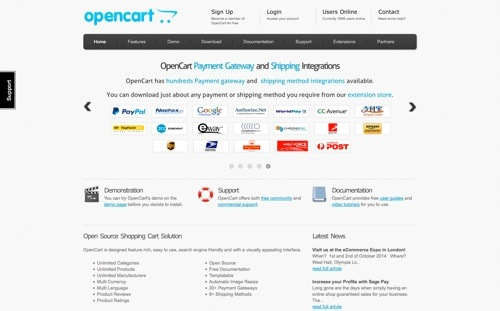
\includegraphics[width=0.5\textwidth]{figuras/cap1/openCartWebsite.jpg}
		\caption{\nameOpenCart \textit{website}\cite{online_OpenCartWebsite}.}
	\end{figure}


	\item \textbf{\namePrestaShop}. Es una solución \ecommerce \opensource, escrita en \php y basada en \textit{Smarty template engine}. \namePrestaShop viene con mas de 310 características integradas y 3500 módulos y \textit{templates}. Cuenta con ventas cruzadas, productos descargables, la exportación de productos, una pagina de pago, envio, descuentos y mucho mas. Descargado mas de 4 millones de veces, \namePrestaShop es usado en 160 países y traducido a 63 idiomas. Tiene mas de 600000 miembros en su comunidad.

	\begin{figure}[h!]
		\centering
		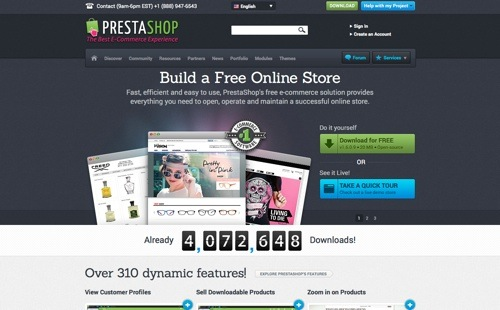
\includegraphics[width=0.5\textwidth]{figuras/cap1/PrestaShopWebsite.jpg}
		\caption{\namePrestaShop \textit{website}\cite{online_PrestaShop}.}
	\end{figure}


	\item \textbf{\nameMagento Community Edition} es una version \free y \opensource de  una plataforma \ecommerce. Los comerciantes pueden acceder a caracteristicas adicionales instalando las extensiones desde el gran \textit{\nameMagento Connect marketplace}. No existe soporte para \nameMagento Community Edition, así que las respuestas a las preguntas técnicas deben ser resultas a través del foro de usuarios. Un detalle, \nameMagento ha anunciado el cierro de su \textit{hosted solution}, \nameMagento Go, por ahora no habrían problemas con Community Edition. \nameMagento Community Edition soporta mas de 200000 sitios de clientes .

	\begin{figure}[h!]
		\centering
		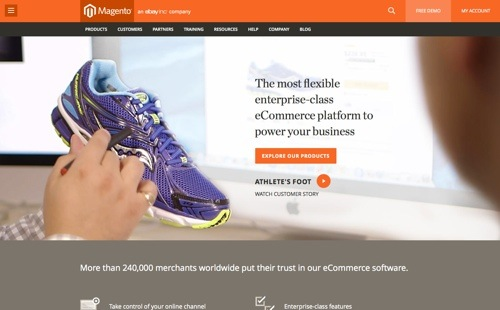
\includegraphics[width=0.5\textwidth]{figuras/cap1/MagentoWebsite.jpg}
		\caption{\nameMagento \textit{website}\cite{online_Magento}.}
	\end{figure}


	\item \textbf{\nameZenCart} es una aplicación \ecommerce \opensource escrita en \php.\nameZenCart \textit{branched} desde el código osCommerce en 2003, con una solución que era mas \textit{template-based}. Tiene mas de 1800 \textit{add-ons} en 16 categorías. La comunidad de apoyo de \nameZenCart tiene aproximadamente 150000 miembros y 200000 \textit{threads}.

	\begin{figure}[h!]
		\centering
		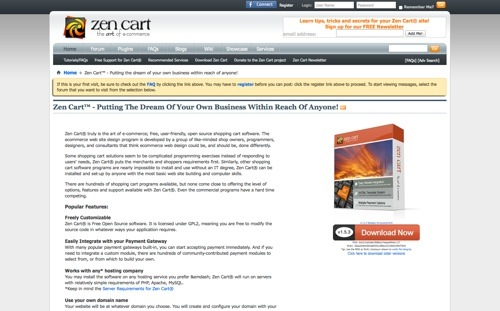
\includegraphics[width=0.5\textwidth]{figuras/cap1/ZenCartWebsite.jpg}
		\caption{\nameZenCart \website\cite{online_ZenCart}.}
	\end{figure}


	\item \textbf{\nameSpreeCommerce} es una solución \ecommerce \opensource  basado en Ruby on Rails. La plataforma modular permite configurar, complementar, o reemplazar cualquier funcionalidad que necesites. \nameSpreeCommerce tiene mas de 45000 tiendas la plataforma al rededor del mundo, incluyendo Chipotle\cite{online_Chipotle}. \nameSpreeCommerce ha sido traducido a más de 30 idiomas.

	\begin{figure}[h!]
		\centering
		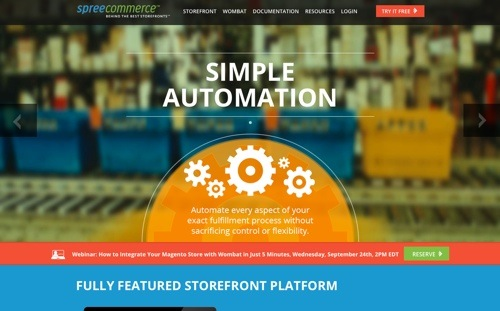
\includegraphics[width=0.5\textwidth]{figuras/cap1/SpreeCommerceWebsite.jpg}
		\caption{\nameSpreeCommerce \website\cite{online_SpreeCommerce}.}
	\end{figure}

	\item \textbf{\nameDrupalCommerce} es una aplicación \ecommerce desarrollado por Commerce Guys. Construido sobre Drupal content management system. \nameDrupalCommerce ofrece un sistema de administración de producto completo, carro de compra varios lenguajes y monedas; y forma de pago. La lista de extension de \nameDrupalCommerce es una integración completamente en\thirdParty para formas de pago,servicios de cumplimiento, aplicaciones de contabilidad, redes sociales y mucho mas. Paquetes de soporte técnico están disponibles por Commerce Guys.

	\begin{figure}[h!]
		\centering
		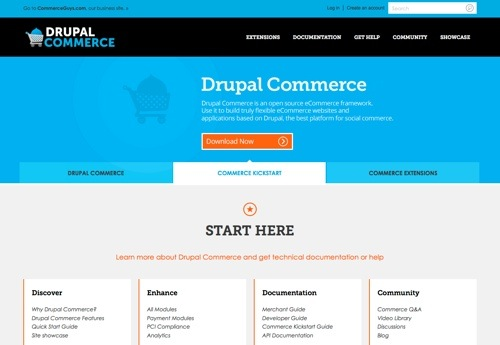
\includegraphics[width=0.5\textwidth]{figuras/cap1/DrupalCommerceWebsite.jpg}
		\caption{\nameDrupalCommerce \website\cite{online_DrupalCommerce}.}
	\end{figure}

	\item \textbf{\nameOsCommerce} (i.e., \opensource \commerce)es uno de las primeras aplicaciones \ecommerce \textit{open-source}. Mas de 7000 \textit{free add-ons} han sido subidos por su comunidad para customizar una  \textit{online store}. \nameOsCommerce es usado por cerca de 13000 sitios registrados. La comunidad de apoyo tiene aproximadamente 280000 miembros los cuales han contribuido con 1.5 millones de \posts en los foros. La comunidad directa juntos con miembros de otra comunidad están disponibles en vivo en el \textit{Chat room}.

	\begin{figure}[h!]
		\centering
		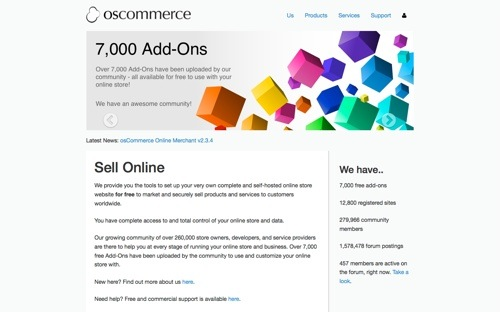
\includegraphics[width=0.5\textwidth]{figuras/cap1/osCommerceWebsite.jpg}
		\caption{\nameOsCommerce \textit{website}\cite{online_osCommerce}.}
	\end{figure}

	\item \textbf{\nameSimpleCart (js)} es un \textit{free} y \textit{open-source} JavaScript \textit{shopping cart}. Con su pequeño tamaño, \nameSimpleCart(js) esta disseñado para mantener simple  y sitions con alto trafico \textit{running fast}. \nameSimpleCart(js) tienen la habilidad de pagar con PayPal Express, Google Checkout, y Amazon Payments. \textit{Email checkout} e integracion con  Authorize.Net llegaran pronto.
	
	\begin{figure}[h!]
		\centering
		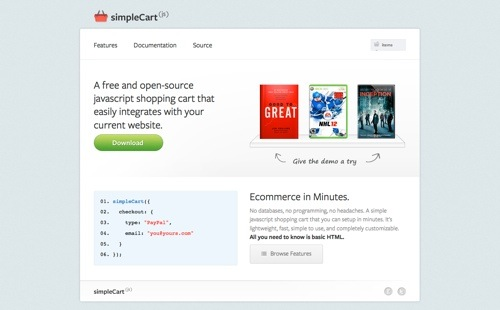
\includegraphics[width=0.5\textwidth]{figuras/cap1/simpleCartWebsite.jpg}
		\caption{\nameSimpleCart \website\cite{online_simpleCart}.}
	\end{figure}

	\item \textbf{\nameWooCommerce} es una aplicación \ecommerce \free \opensource que permite a los comerciantes transformar \wordPress \sites en \stores. \nameWooCommerce fue desarrollado por \wooThemes desde un \fork de \nameJigoshop. \nameWooCommerce tiene una larga variedad de  \plugins y  \themes de \wooThemes, como de sitios \thirdParty tales como \themeForest \cite{online_ThemeForest} y \codeCanyon \cite{online_CodeCanyon}. Con cerca de 4.5 millones de descargas desde \wordPressOrg\cite{online_WordPress}, \nameWooCommerce es una solución \ecommerce muy popular para \wordPress. Para obtener el soporte oficial de \wooThemes, es necesario comprar un producto. De otra manera, obtener ayuda desde la comunidad activa del foro.

	\begin{figure}[h!]
		\centering
		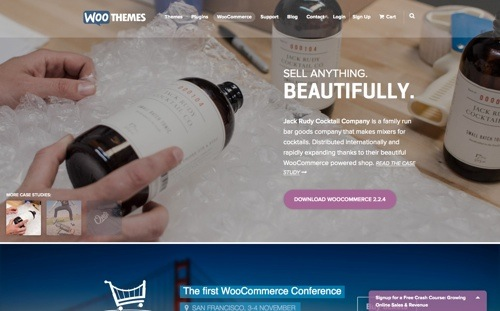
\includegraphics[width=0.5\textwidth]{figuras/cap1/WooCommerceWebsite.jpg}
		\caption{\nameWooCommerce \website\cite{online_WooCommerce}.}
	\end{figure}

	\item \textbf{\nameWPECommerce} es otra aplicación popular obtenida desde la conversión del  sitio \wordPress a una \ecommerce \store.\nameWPECommerce tiene cerca de 3 millones de descarga de \plugin desde \wordPressOrg\cite{online_WordPress}. Usa el propio \html y \css y obtén el control completo sobre la vista y la experiencia de tu \online \store. \nameWPECommerce tiene una gran variedad de características estándar, incluyendo \textit{ multi-tier pricing} para descuentos por cantidad e integración con redes sociales para \marketing. Para soporte, hay tutoriales en video y un foro en \wordPressOrg, también como consultantes de características para ayuda profesional.

	\begin{figure}[h!]
		\centering
		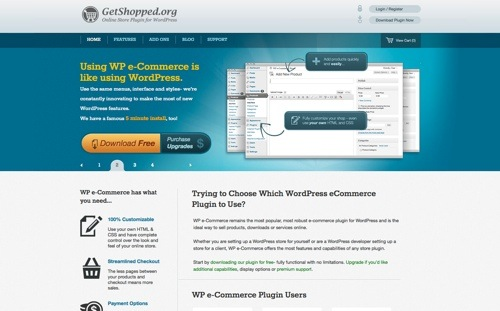
\includegraphics[width=0.5\textwidth]{figuras/cap1/WPECommerceWebsite.jpg}
		\caption{\nameWPECommerce \website\cite{online_WPECommerce}.}
	\end{figure}

	\item \textbf{\nameJigoshop} es una solución \ecommerce \textit{free} y \opensource basado en \wordPress. Liberado en 2011, \nameJigoshop es el predecesor para \nameWooCommerce. \nameJigoshop tiene mas de 30   \themes, 100 extensiones, y tres \theme \frameworks. \nameJigoshop es  \free, así como el soporte a \wordPressOrg. Sin embargo, el acceso a la comunidad de \textit{Jigoshop.com} comienza desde \$40 por mes.

	\begin{figure}[h!]
		\centering
		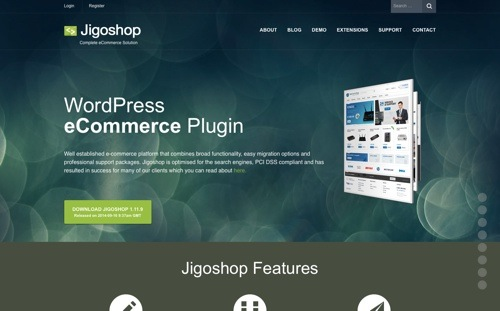
\includegraphics[width=0.5\textwidth]{figuras/cap1/JigoshopWebsite.jpg}
		\caption{\nameJigoshop \textit{website}\cite{online_Jigoshop}.}
	\end{figure}

\end{itemize}

\begin{table}[h!]
    \tiny
   
%\begin{tabular}{ |C{0.3\paperwidth}|C{0.3\paperwidth}| }
\begin{tabular}{ |l|c|c|c|c|c| }

\hline
	&
	\textit{Free database backend support}&
	Language&
	\textit{\gloss{waf}}&
	License&

\\ \hline
	\nameOpenCart &
	MySQL&
	PHP&
	&
	GPLv3&
	
\\ \hline
	\namePrestaShop &
	MySQL&
	PHP&
	&
	Open Software License&
	
\\ \hline
	\nameMagento &
	MySQL&
	PHP&
	Zend Framework\cite{online_zend_framework}&
	Open Software License&
	
\\ \hline
	\nameZenCart &
	&
	&
	&
	&
 
\\ \hline
	\nameSpreeCommerce &
	MySQL, PostgreSQL, SQLite3&
	Ruby\cite{online_ruby_language}&
	Ruby on Rails\cite{online_ruby_rails}&
	New BSD License&

\\ \hline
	\nameDrupalCommerce &
	MySQL, PostgreSQL, SQLite3&
	PHP&
	Drupal\cite{online_drupal}&
	GNU GPL&
	
\\ \hline
	\nameOsCommerce &
	&
	&
	&
	&

\\ \hline
	\nameSimpleCart &
	&
	&
	&
	&
	
\\ \hline
	\nameWooCommerce &
	MySQL&
	PHP&
	WordPress\cite{online_wordpress}&
	GNU GPL&
	
\\ \hline
	\nameWPECommerce &
	&
	&
	&
	&
	
\\ \hline
	\nameJigoshop &
	MySQL&
	PHP&
	WordPress\cite{online_wordpress}&
	GNU GPL&
	
\\ \hline
\end{tabular}
    \caption{ Comparación entre diferentes opciones \ecommerce}
    \label{tab:wide_table}
\end{table}

\begin{table}[h!]
    \tiny
   
%\begin{tabular}{ |C{0.3\paperwidth}|C{0.3\paperwidth}| }
\begin{tabular}{ |l|c|c|c|c| }
\hline
	&
	traider\cite{online_Traider}&
	ReactionCommerce\cite{online_reactionCommerce}&
	NodeShop\cite{online_NodeShop}&
	Forward\cite{online_Forward}
 
\\ \hline
	Tecnología &
	bootstrap, nodejs and mongodb &
	Nodejs, Meteor, Mongodb, CoffeScript, Bootstrap, Docker&
	&
	

\\ \hline
	Mobile &
	&
	&
	&
\\ \hline
	version &
	&
	&
	0.06 ( 21/08/2013 )&
	0.1

\\ \hline
\end{tabular}
    \caption{ Resumen tecnologías entre diferentes opciones \textit{e-Commerce}}
    \label{tab:resume_technology_ecommerce}
\end{table}

\section{Tecnologías }\label{cap:estadoArte:tecnologias}

\begin{itemize}
	\item \textbf{\mongodb} (from "humongous") is an open-source document database, and the leading \nosql database. Written in C++ \cite{technology_mongodb}.
	
%	\item \textbf{Angularjs} \cite{technology_angularjs}
	\item \textbf{\meteor} 
	
	\item \textbf{\bootstrap} is the most popular HTML, CSS, and JS framework for developing responsive, mobile first projects on the web \cite{technology_bootstrap}.
	
	\item \textbf{\nodejs} is a platform built on Chrome's JavaScript runtime for easily building fast, scalable network applications. Node.js uses an event-driven, non-blocking I/O model that makes it lightweight and efficient, perfect for data-intensive real-time applications that run across distributed devices \cite{technology_nodejs}.
	
	\item \textbf{\coffeescript} is a little language that compiles into JavaScript. Underneath that awkward Java-esque patina, JavaScript has always had a gorgeous heart. CoffeeScript is an attempt to expose the good parts of JavaScript in a simple way.
	
	The golden rule of \coffeescript is: "It's just JavaScript". The code compiles one-to-one into the equivalent JS, and there is no interpretation at runtime. You can use any existing JavaScript library seamlessly from CoffeeScript (and vice-versa). The compiled output is readable and pretty-printed, will work in every JavaScript runtime, and tends to run as fast or faster than the equivalent handwritten JavaScript \cite{technology_coffeescript}.
	
	\item \textbf{\grunttool} \cite{technology_gruntjs}
	
	\item \textbf{\docker} es una platarma \opensource y \sysadmins para construir,  \cite{technology_docker}.
	%is an open platform for developers and sysadmins to build, ship, and run distributed applications. Consisting of Docker Engine, a portable, lightweight runtime and packaging tool, and Docker Hub, a cloud service for sharing applications and automating workflows, Docker enables apps to be quickly assembled from components and eliminates the friction between development, QA, and production environments. As a result, IT can ship faster and run the same app, unchanged, on laptops, data center VMs, and any cloud\cite{technology_docker}.
	
\end{itemize}



\begin{table}[h!]
    \tiny
   
%\begin{tabular}{ |C{0.3\paperwidth}|C{0.3\paperwidth}| }
\begin{tabular}{ |L{0.1\paperwidth}|L{0.3\paperwidth}|L{0.3\paperwidth}|}
\hline
	\ecommerce&
	SQL Databases &
	NoSQL Databases
 
\\ \hline
	El \textit{schema} de los productos varia&
	\textit{Schema} rigido&
	\textit{Schema} flexible
\\ \hline
	Necesita escalar&
	&
	
\\ \hline
	Transacciones&
	&
	
\\ \hline
\end{tabular}
    \caption{ \nosql vs. \sql en relación a \ecommerce}
    \label{tab:SQL_vs_noSQL_summary}
\end{table}

	\subsection{ \textit{Full-Stack} JavaScript }
	
	%Before digging into Node.js, you might want to read up on the benefits of using JavaScript across the stack which unifies the language and data format (JSON), allowing you to optimally reuse developer resources. As this is more a benefit of JavaScript than Node.js specifically, we won’t discuss it much here. But it’s a key advantage to incorporating Node in your stack.



Recapitulando, he demostrado que las soluciones actuales de \ecommerce pueden ser considerablemente mejoradas utilizando la tecnología actualmente presente. 
Importante notar que solo estoy ofreciendo una mejor solución a lo que ya existe, en ningún caso indico la solución que presento es la mejor posible. No se ha realizado un estudio sobre todas las opciones disponibles del mercado. Sin embargo esta solución ofrece

speed
scalability
flexibility
performance
